% !TeX root = ../dokumentation.tex

\addchap{\langanhang}

{\Large
\begin{enumerate}[label=\Alph*.]
	\item Screenshot NameNode Web-Interface
	\item DVD Inhalt
	\item DVD 
\end{enumerate}
}
\pagebreak

\section*{A. Screenshot NameNode Web-Interface}\label{sec:ScreenNameNodeWeb}
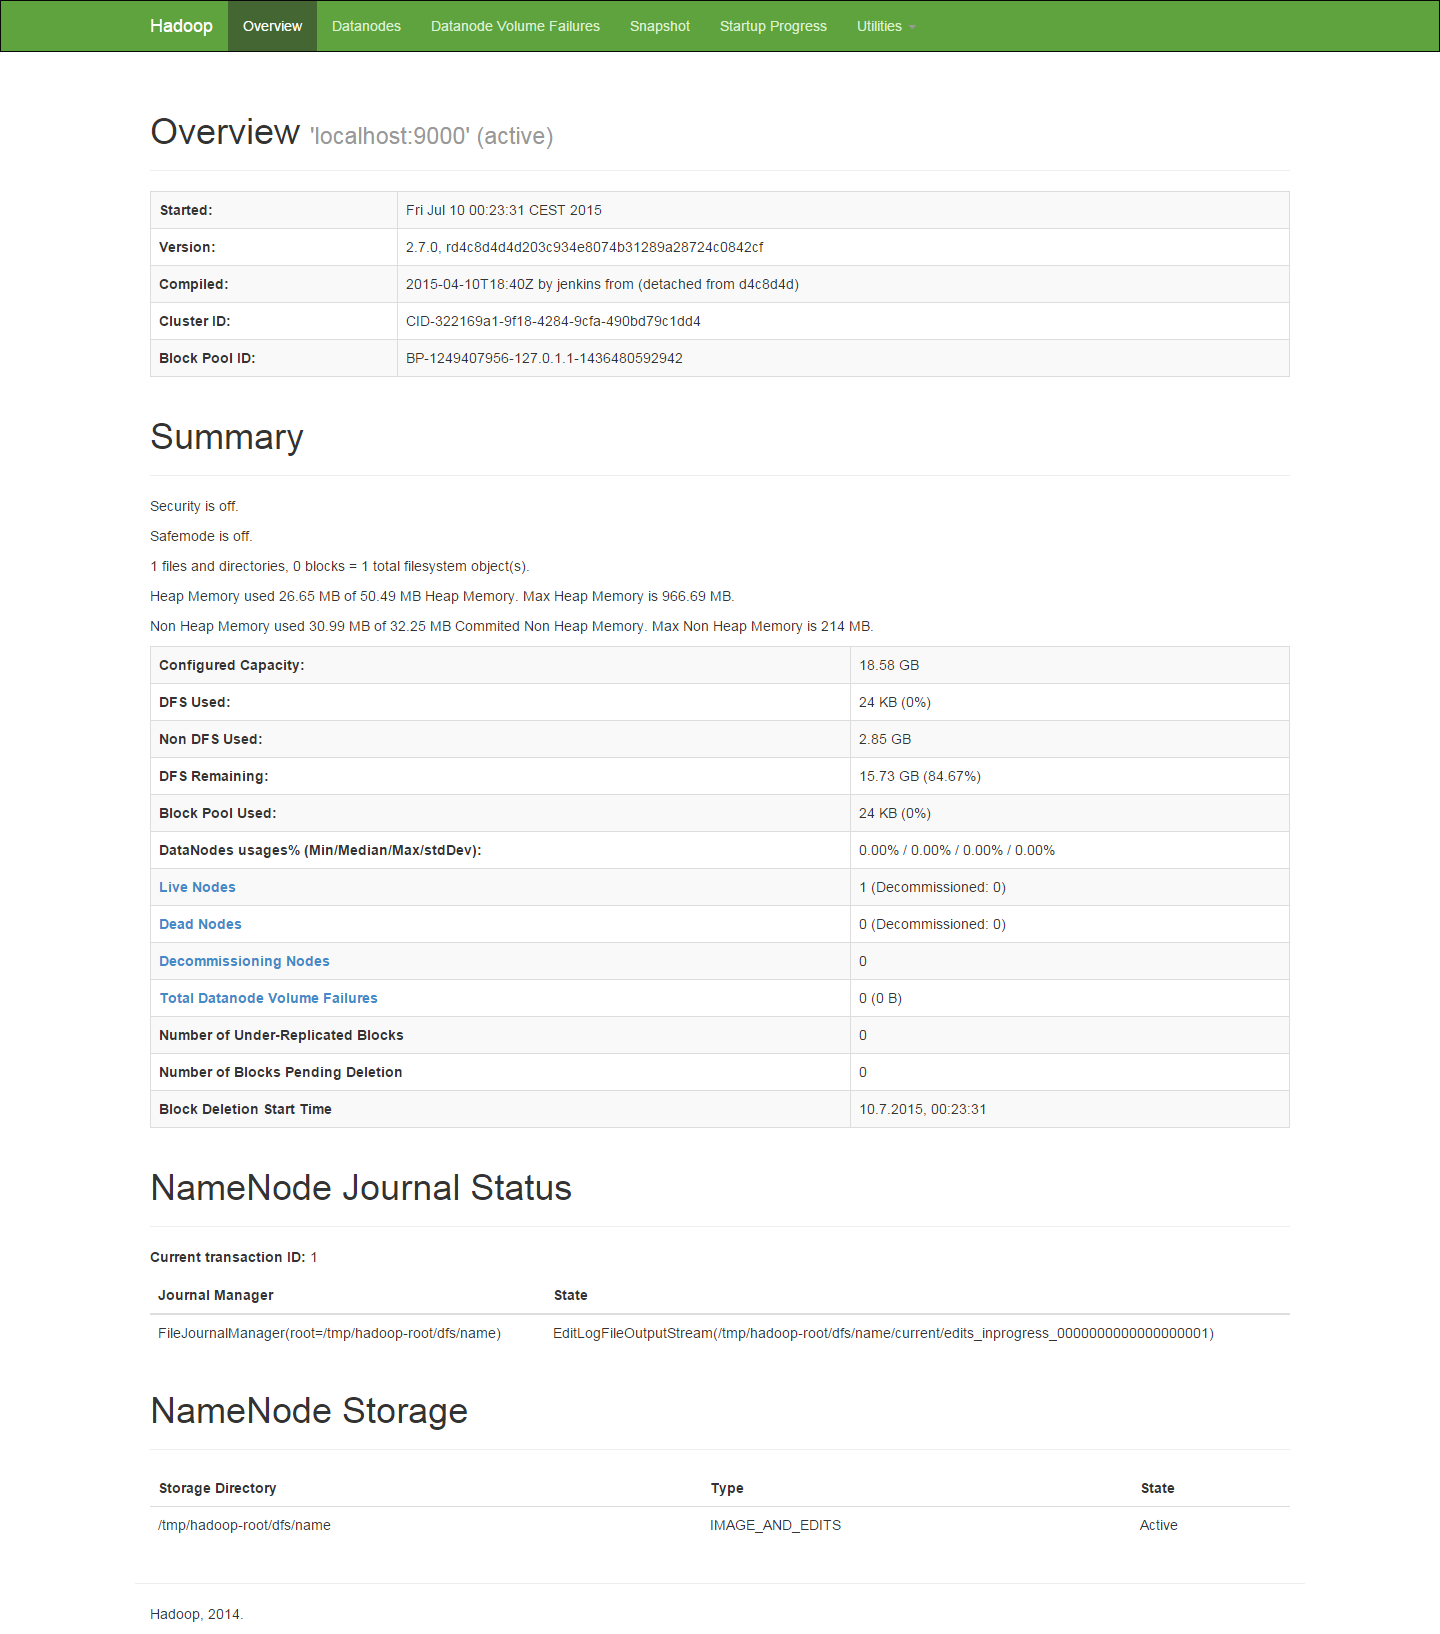
\includegraphics[width=1\textwidth]{NameNodeWebInterface.png}
\pagebreak

\section*{C. DVD Inhalt}
\begin{tabbing}
	mm \= mm \= mm \= mmmmmmmmmmmmmmmmmm \= \kill
	$\vdash$ \textbf{Anwendung/} \\ 
	| \> -- pom-xml \> \> \> $\Rightarrow$ \textit{Maven POM Datei} \\
	| \> $\vdash$ \textbf{conf/} \> \> \> $\Rightarrow$ \textit{*.properties Dateien für Konfiguration} \\
	| \> $\vdash$ \textbf{src/} \> \> \> $\Rightarrow$ \textit{Quellcode Dateien} \\
	| \> $\vdash$ \textbf{target/} \\
	| \> | \> -- Logfileanalyzer-1.0-SNAPSHOT.jar \> \> $\Rightarrow$ \textit{Ausführtbare JAR-Datei} \\
	| \> | \> $\vdash$ \textbf{site/apidocs/} \> \> $\Rightarrow$ \textit{JavaDoc für Browser} \\
	| \\
	$\vdash$ \textbf{Literatur/} \> \> \> \> $\Rightarrow$ \textit{PDF Literatur \& E-Books} \\
	$\vdash$ \textbf{Praesentationen/} \\
	| \> -- Abschlusspraesentation.pptx \> \> \> $\Rightarrow$ \textit{Präsentation vom 21. August 2015} \\
	| \> -- Abschlusspraesentation.pdf \\
	| \> -- Kickoffpraesentation.pptx \> \> \> $\Rightarrow$ \textit{Präsentation vom 03. Juni 2015} \\
	| \> -- Kickoffpraesentation.pdf \\
	| \\
	$\vdash$ \textbf{Sonstiges/} \\
	| \> -- LineareRegression.xlsx \> \> \> $\Rightarrow$ \textit{Berechnung der linearen Regression} \\
	| \\
	$\vdash$ \textbf{Latex-Files/} \> \> \> \> $\Rightarrow$ \textit{Editierbare \LaTeX~Dateien der Arbeit}\\ %\llcorner
	\> -- bibliographie.bib \> \> \> $\Rightarrow$ \textit{Literaturverzeichnis} \\
	\> -- dokumentation.pdf \> \> \> $\Rightarrow$ \textit{Bachelorarbeit als PDF} \\
	\> -- dokumentation.tex \> \> \> $\Rightarrow$ \textit{Hauptdokument} \\
	\> -- einstellungen.tex \> \> \> $\Rightarrow$ \textit{Einstellungen} \\
	\> $\vdash$  \textbf{ads/}   	\> \> \> $\Rightarrow$ \textit{Header, Glosar, Abkürzungen, etc.}\\
	\> $\vdash$  \textbf{content/}  \> \> \> $\Rightarrow$ \textit{Kapitel}\\
	\> $\vdash$  \textbf{images/}   \> \> \> $\Rightarrow$ \textit{Bilder}\\
	\> $\vdash$  \textbf{lang/}  \> \> \> $\Rightarrow$ \textit{Sprachdateien für \LaTeX~Template}\\
	\> 
\end{tabbing}
